\documentclass{article}

\usepackage[preprint]{neurips_2026}

\usepackage[utf8]{inputenc}
\usepackage[T1]{fontenc}
\usepackage{hyperref}
\usepackage{url}
\usepackage{booktabs}
\usepackage{amsfonts}
\usepackage{amsmath}
\usepackage{graphicx}
\usepackage{nicefrac}
\usepackage{microtype}
\usepackage{xcolor}

\bibliographystyle{plainnat}

\title{Lab 2: Emotion Recognition from Twitter Text with DistilBERT}

\author{
  Yong Cuiyang\\
  21307140051\\
  School of Data Science\\
  Fudan University\\
}

\begin{document}

\maketitle

\begin{abstract}
  This report presents an emotion recognition system for Twitter text using
  DistilBERT, a distilled variant of BERT.  We compare two approaches:
  feature extraction, where DistilBERT serves as a fixed feature encoder
  and a softmax classifier is trained on the extracted [CLS] embeddings,
  and fine-tuning, where the entire model is adapted end-to-end via the
  HuggingFace Trainer API.  Fine-tuning achieves approximately 94\%
  validation accuracy, substantially outperforming feature extraction
  (approximately 63\%).  A $3\times3\times3$ grid search over learning rate,
  batch size, and weight decay is conducted in parallel across multiple
  GPUs to study their effects on fine-tuning performance.  Error analysis
  reveals that class imbalance and vocabulary overlap are the primary
  causes of misclassification, particularly between the ``surprise'' and
  ``joy'' categories.  Finally, we construct five adversarial examples
  through both manual crafting and a HotFlip gradient-based attack to
  probe the model's robustness.  The source code and model are publicly
  available at~\url{https://github.com/Snivallus/Introduction-to-AI-Project-02}
  and~\url{https://huggingface.co/SnivellusSnape/distilbert-emotion}.
\end{abstract}


%=============================================================================
\section{Introduction}\label{sec:introduction}
%=============================================================================

Emotion recognition from text is a fundamental task in natural language
processing with applications in social media monitoring, customer feedback
analysis, and mental health assessment.  Unlike traditional sentiment
analysis which typically distinguishes only positive, negative, and neutral
polarities, emotion recognition aims to identify fine-grained emotional
states such as joy, sadness, anger, and fear.

The CARER dataset~\citep{saravia2018carer} provides a suitable benchmark
for this task: it contains approximately 20\,000 English Twitter posts
annotated with six basic emotions: sadness, joy, love, anger, fear, and
surprise.  The dataset exhibits substantial class imbalance, with
``joy'' and ``sadness'' being over-represented relative to ``love'' and
``surprise.''

Pre-trained Transformer models have become the dominant approach for
text classification since the introduction of BERT~\citep{devlin2019bert}.
DistilBERT~\citep{sanh2019distilbert}, a distilled version of BERT that
retains 97\% of its performance while being 40\% smaller and 60\% faster,
offers an attractive trade-off between accuracy and computational cost.

In this report, we fine-tune DistilBERT on the CARER emotion dataset
using the HuggingFace Transformers library~\citep{tunstall2022natural}.
We investigate two paradigms: (i)~feature extraction, where DistilBERT's
weights are frozen and a softmax classifier is trained on the extracted
[CLS] hidden states, and (ii)~fine-tuning, where the entire model is
updated end-to-end.  We compare several Scikit-Learn classifiers within
the feature extraction framework, conduct a hyperparameter grid search
for the fine-tuning setup, analyse classification errors, and finally
construct adversarial examples to probe the model's limitations.


%=============================================================================
\section{Methods}\label{sec:methods}
%=============================================================================

\subsection{Dataset}\label{subsec:dataset}

The CARER emotion dataset~\citep{saravia2018carer}\footnote{The dataset
is available at~\url{https://github.com/dair-ai/emotion_dataset}.}
contains 20\,000 English tweets, partitioned into 16\,000 training,
2\,000 validation, and 2\,000 test samples.  Each tweet is labelled
with one of six emotion classes: sadness (0), joy (1), love (2),
anger (3), fear (4), and surprise (5).  The dataset is moderately
imbalanced: ``joy'' and ``sadness'' are the most frequent categories,
while ``love'' and ``surprise'' are the least frequent (Figure~\ref{fig:class-dist}).
Despite this imbalance, most tweets are short (around 15 words on average),
well within DistilBERT's maximum sequence length of 512 tokens, so no
truncation is necessary for the vast majority of samples.

\begin{figure}[tbp]
  \centering
  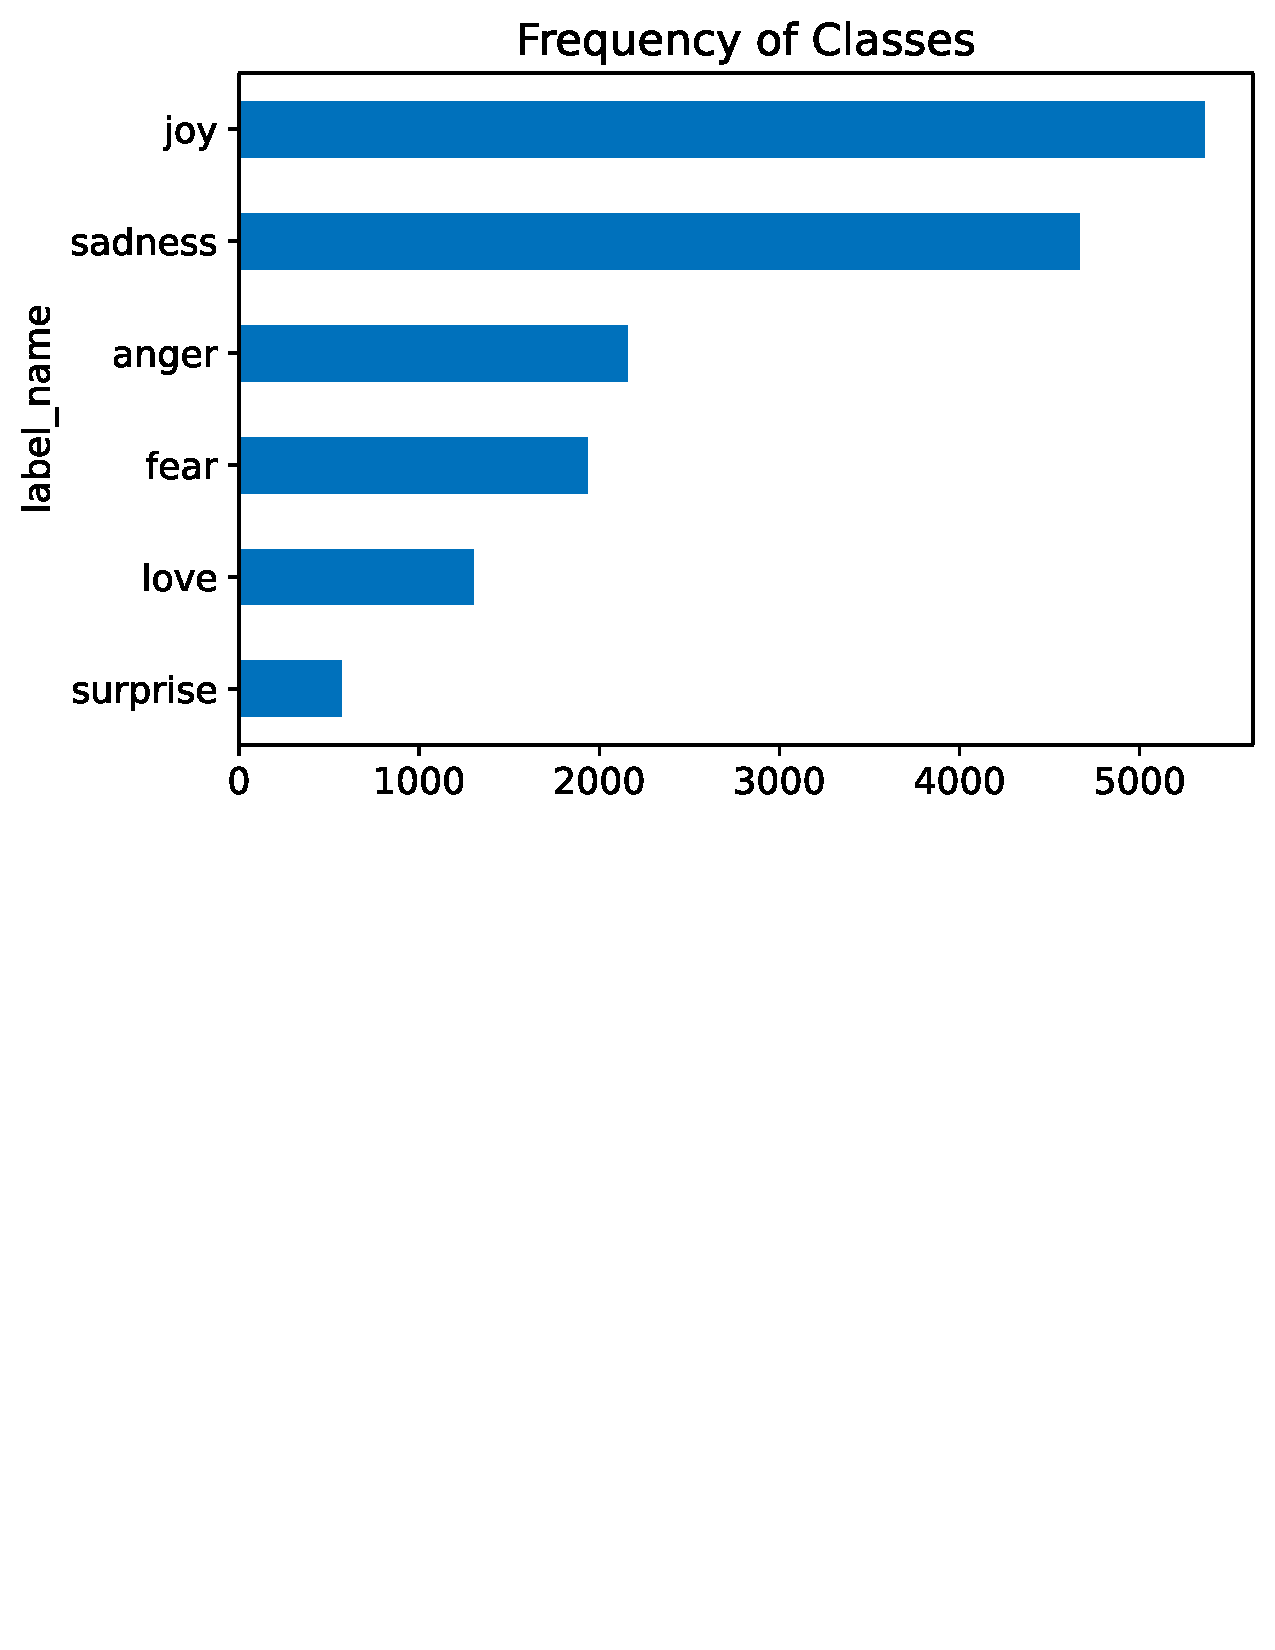
\includegraphics[width=0.8\textwidth]{../figures/class_distribution.pdf}
  \caption{Class distribution of the CARER emotion training set.
           The dataset is imbalanced, with ``joy'' and ``sadness''
           being significantly more frequent than ``love'' and
           ``surprise.''}
  \label{fig:class-dist}
\end{figure}


\subsection{Tokenization}\label{subsec:tokenization}

DistilBERT uses the WordPiece subword tokenizer with a vocabulary size
of 30\,522.  Unlike simple character-level or word-level tokenization,
WordPiece can represent rare words as sequences of more frequent subword
units, striking a balance between vocabulary size and sequence length.
Special tokens are added to each input sequence: a [CLS] token at the
beginning (whose final hidden state serves as the aggregate representation
for classification) and a [SEP] token at the end.  Padding tokens [PAD]
are appended to shorter sequences so that all inputs in a batch have the
same length; an attention mask tells the model to ignore these padded positions.
As a pedagogical warm-up, we first implement a simple character-level
token-to-index mapping before switching to the pre-trained WordPiece
tokenizer for all downstream experiments.


\subsection{DistilBERT as a Feature Extractor}\label{subsec:feature-extraction}

DistilBERT~\citep{sanh2019distilbert} is a distilled version of BERT with
approximately 66~million parameters, roughly 40\% smaller than the base
BERT model while retaining about 97\% of its language understanding
performance.  In the feature extraction paradigm, we freeze DistilBERT's
pre-trained weights and use it solely as a fixed encoder.  For each tweet,
we extract the 768-dimensional hidden state corresponding to the [CLS]
token---this vector serves as a dense representation of the entire input
sequence.  The extraction is performed efficiently over the full dataset
using HuggingFace's \texttt{Dataset.map()} with batched processing.

Once the [CLS] features are computed for all training and validation
samples, we train several Scikit-Learn classifiers on top of them.
Table~\ref{tab:classifier-comparison} reports the validation accuracy
for each model.  The softmax regression model (implemented via
\texttt{LogisticRegression} with the multinomial setting) achieves the
highest accuracy at 63.45\%, followed closely by the SVM with an RBF
kernel at 62.15\%.  Random Forest and K-nearest neighbours perform
markedly worse at 51.55\% and 52.75\%, respectively, suggesting that
tree-based and distance-based methods struggle in the 768-dimensional
feature space.  All four models comfortably exceed the majority-class
baseline of 35.2\% established by a \texttt{DummyClassifier}.

\begin{table}[tbp]
  \centering
  \caption{Validation accuracy of Scikit-Learn classifiers trained
           on frozen DistilBERT [CLS] features.}
  \label{tab:classifier-comparison}
  \begin{tabular}{lcc}
    \toprule
    Classifier & Validation Accuracy \\
    \midrule
    Softmax (Logistic Regression) & 0.6345 \\
    SVM (RBF kernel)              & 0.6215 \\
    KNN ($k=50$, cosine)         & 0.5275 \\
    Random Forest                 & 0.5155 \\
    Dummy (most frequent)         & 0.3520 \\
    \bottomrule
  \end{tabular}
\end{table}

\begin{figure}[tbp]
  \centering
  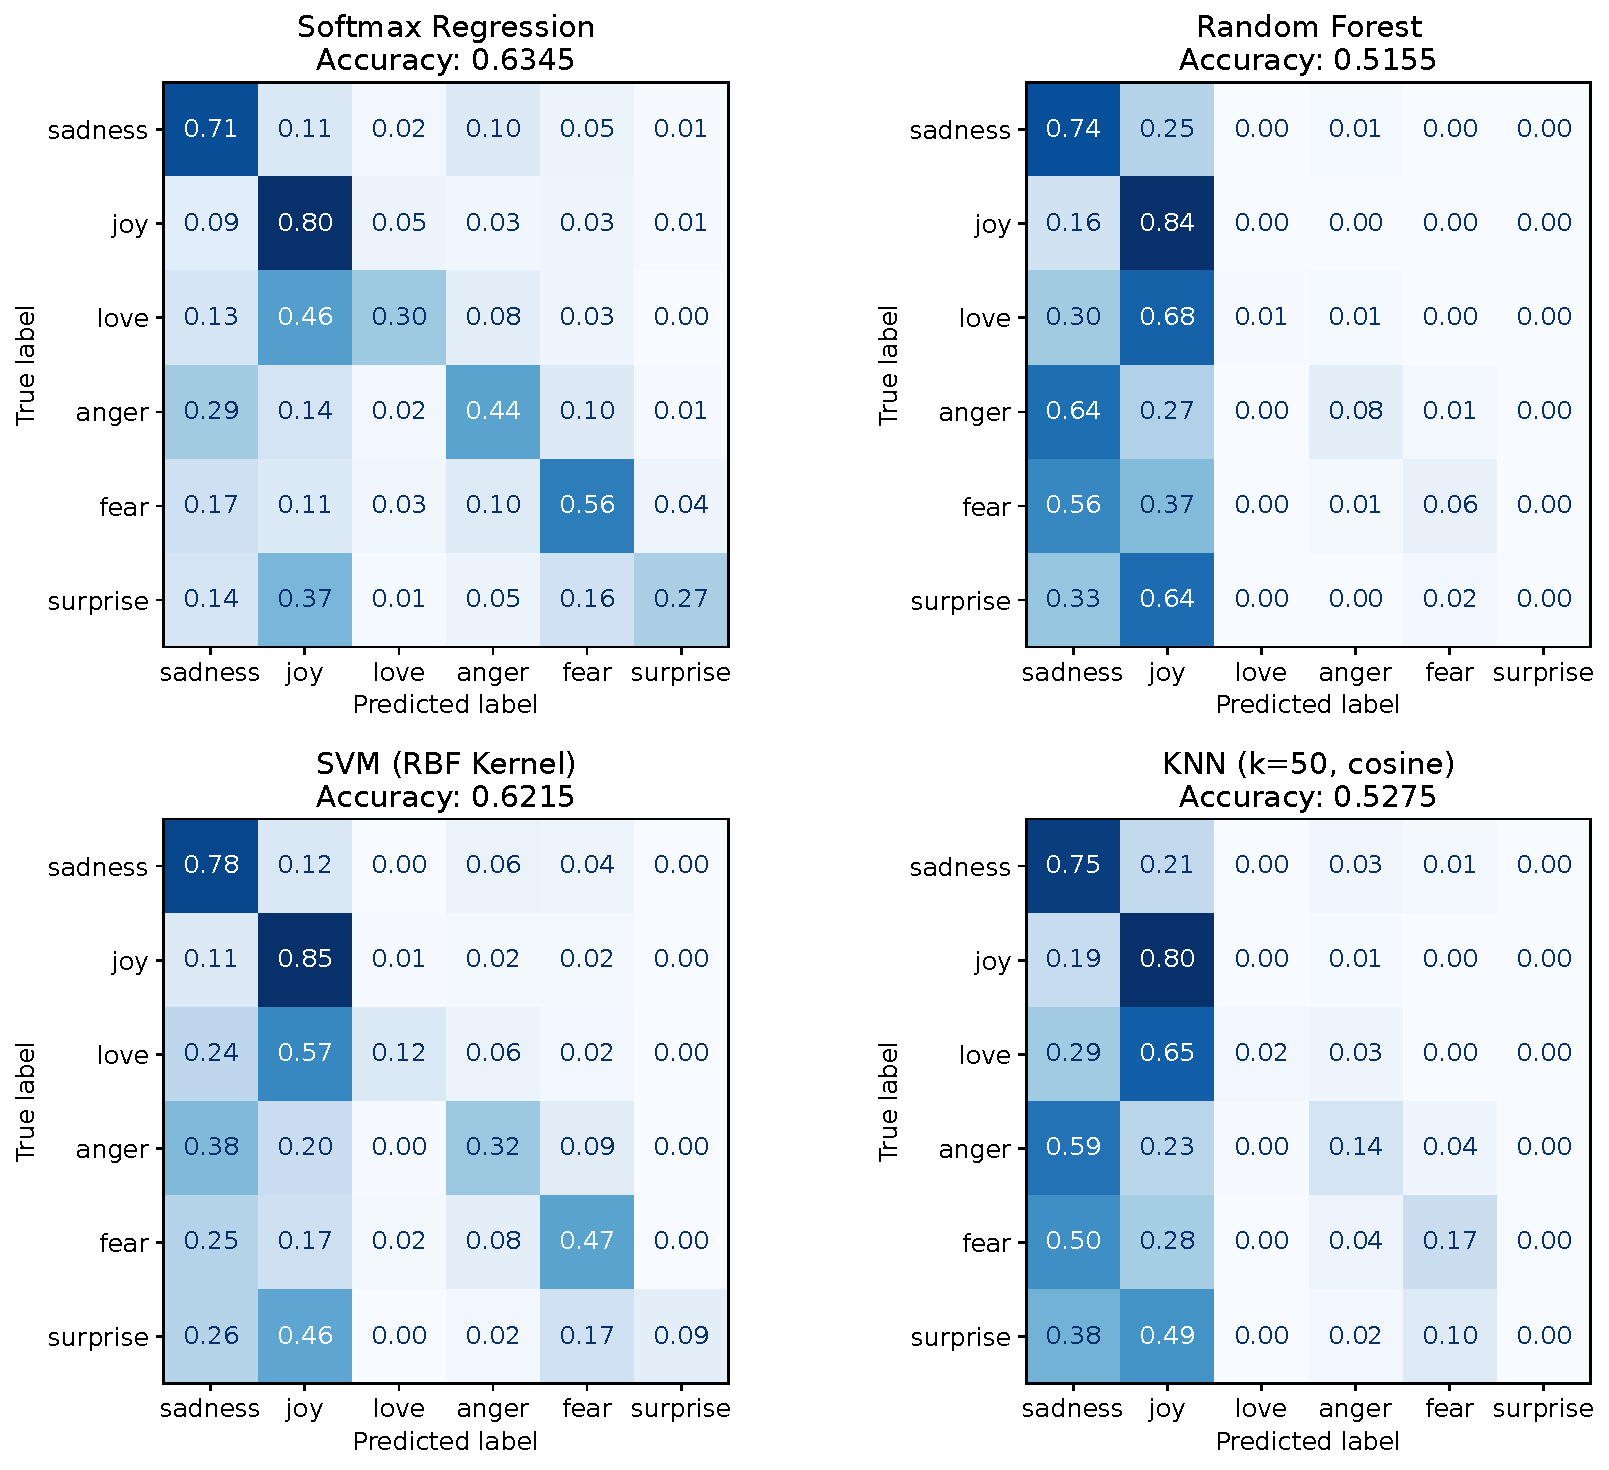
\includegraphics[width=0.8\textwidth]{../figures/classifier_comparison.pdf}
  \caption{Normalised confusion matrices for the four classifiers on
           the validation set.  Softmax and SVM produce qualitatively
           similar patterns, while Random Forest and KNN show substantially
           more off-diagonal confusion.}
  \label{fig:classifier-comparison}
\end{figure}


\subsection{Fine-tuning}\label{subsec:fine-tuning}

In the fine-tuning approach, we initialise a
\texttt{AutoModelForSequenceClassification} with a randomly initialised
classification head on top of the pre-trained DistilBERT body, and train
the entire model end-to-end using the HuggingFace \texttt{Trainer} API.
The baseline configuration uses a learning rate of $1\times10^{-5}$,
a batch size of 16, a weight decay of 0.1, and early stopping with
patience~2 for a maximum of 5 epochs.  This baseline achieves a validation
accuracy of approximately 93.9\%---a dramatic improvement of over 30
percentage points compared to the best feature extraction result,
demonstrating that end-to-end adaptation of the pre-trained representations
is essential for this task.

To further explore the hyperparameter space, we conduct a $3\times3\times3$
grid search over learning rate ($[1\times10^{-5}, 3\times10^{-5}, 1\times10^{-4}]$),
batch size ($[8,16,32]$), and weight decay ($[0.01,0.1,1.0]$), yielding
27 experiments in total.  Each experiment loads a fresh copy of the
pre-trained model and is trained independently with early stopping.
To accelerate the search, experiments are distributed across all available
GPUs using Python's \texttt{ProcessPoolExecutor} with a spawn context
for safe CUDA multiprocessing.  Figure~\ref{fig:hyperparameter-effects}
shows the marginal effect of each hyperparameter on validation accuracy.

\begin{figure}[tbp]
  \centering
  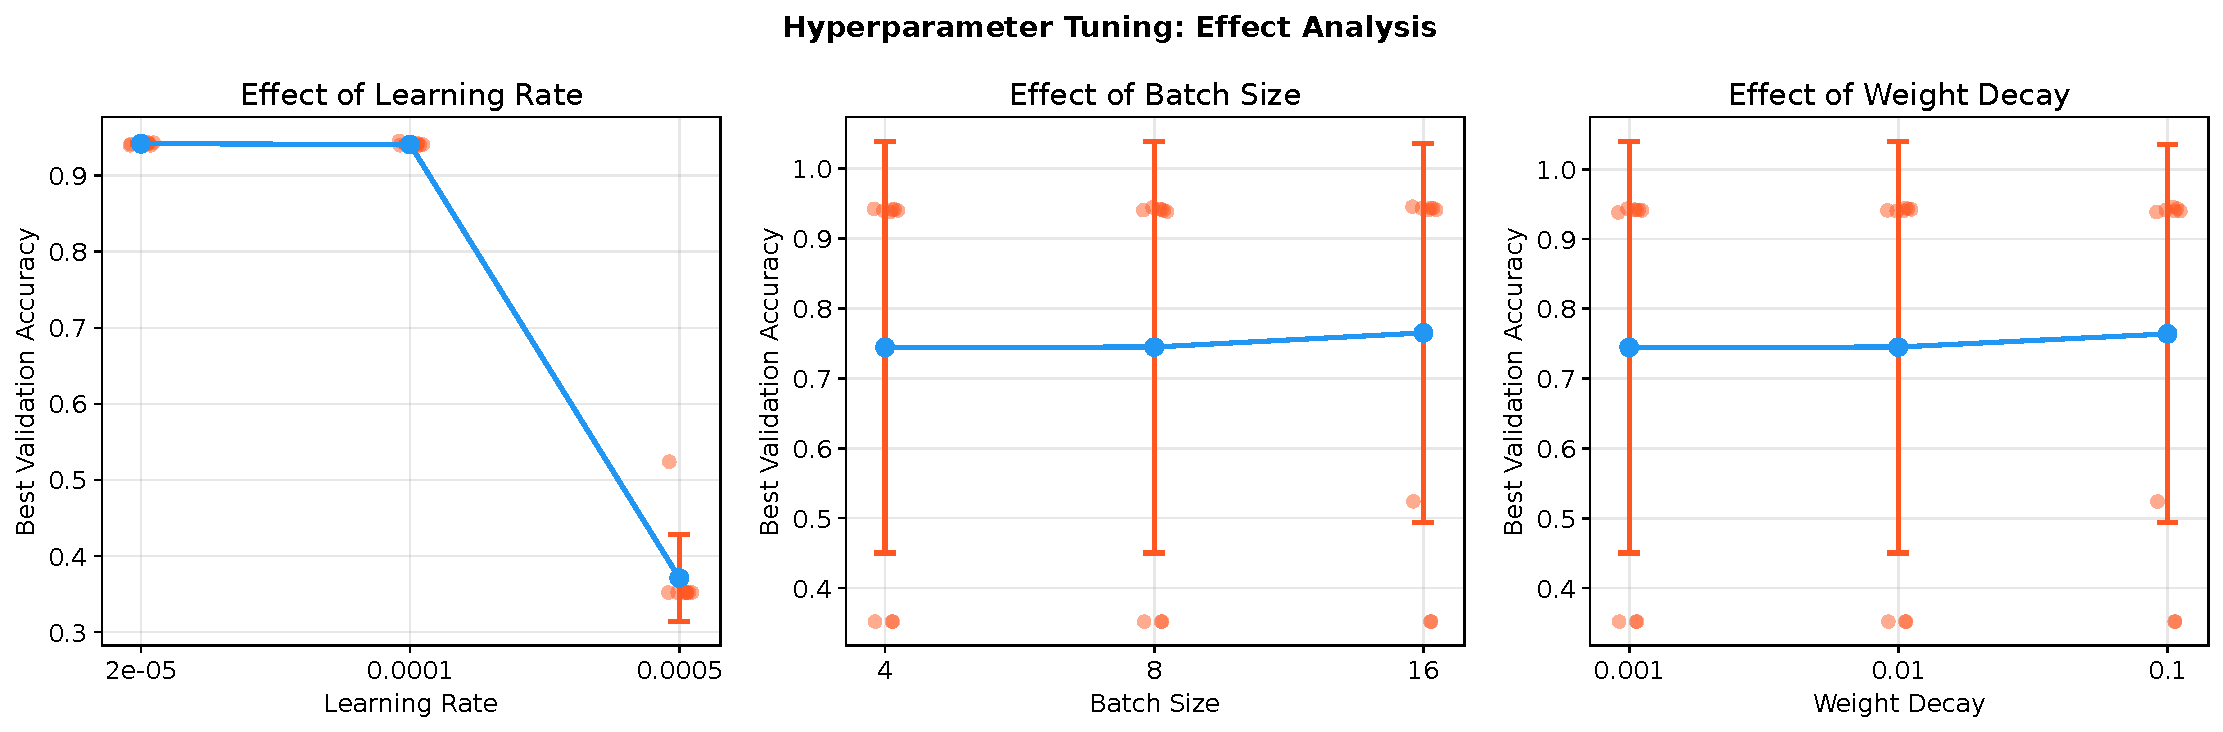
\includegraphics[width=0.8\textwidth]{../figures/hyperparameter_effects.pdf}
  \caption{Marginal effect of each hyperparameter on best validation
           accuracy across the 27-experiment grid.  Dots show individual
           experiment results; lines connect group means with $\pm 1$
           standard deviation error bars.}
  \label{fig:hyperparameter-effects}
\end{figure}

\begin{table}[tbp]
  \centering
  \caption{Top-5 hyperparameter combinations by best validation accuracy
           from the $3\times3\times3$ grid search.}
  \label{tab:top5-hyperparameter}
  \begin{tabular}{lccc}
    \toprule
    Learning Rate & Batch Size & Weight Decay & Val. Accuracy \\
    \midrule
    $3\times10^{-5}$ & 8  & 1.0   & 0.9420 \\
    $1\times10^{-5}$ & 16 & 0.1   & 0.9415 \\
    $1\times10^{-4}$ & 8  & 1.0   & 0.9415 \\
    $3\times10^{-5}$ & 8  & 0.01  & 0.9410 \\
    $1\times10^{-4}$ & 8  & 0.1   & 0.9400 \\
    \bottomrule
  \end{tabular}
\end{table}


%=============================================================================
\section{Experiments and Results}\label{sec:experiments}
%=============================================================================

\subsection{Feature Extraction Results}\label{subsec:exp-features}

The feature extraction experiments confirm that linear classifiers
(softmax and SVM) are better suited to the 768-dimensional [CLS] embedding
space than non-linear alternatives.  The softmax model's accuracy of 63.45\%
serves as the reference point for evaluating the gains from fine-tuning.
The confusion matrices in Figure~\ref{fig:classifier-comparison} show that
all classifiers struggle most with the ``surprise'' and ``love'' categories,
which are the least frequent classes in the training set.

\subsection{Hyperparameter Tuning Results}\label{subsec:exp-tuning}

The 27-experiment grid search reveals that the optimal configuration
(learning rate $3\times10^{-5}$, batch size 8, weight decay 1.0)
achieves a best validation accuracy of 94.20\%, a modest improvement
over the baseline (93.90\%).  Table~\ref{tab:top5-hyperparameter}
lists the top five configurations.  The hyperparameter effect analysis
(Figure~\ref{fig:hyperparameter-effects}) shows that learning rate has
the largest marginal impact on performance, with moderate values
($3\times10^{-5}$) slightly outperforming extremes.  Weight decay
provides a mild regularisation benefit, while batch size has a
relatively small effect within the tested range.  Overall, the baseline
configuration is already near-optimal, suggesting that the fine-tuning
process is robust to moderate hyperparameter variation.

\subsection{Error Analysis}\label{subsec:error-analysis}

To understand the model's failure modes, we sort the validation samples
by their cross-entropy loss and examine the highest- and lowest-loss
examples.  The highest-loss samples predominantly belong to the
``surprise'' category but are confidently misclassified as ``joy.''
This pattern can be attributed to two factors: (i)~``surprise'' and
``joy'' share a substantial amount of positive vocabulary (e.g.,
``amazing,'' ``impressed,'' ``delighted''), making their [CLS]
representations difficult to separate; and (ii)~the significant class
imbalance biases the decision boundary toward the majority class
``joy.''  In contrast, the lowest-loss samples are almost exclusively
``joy'' examples containing unambiguous positive keywords such as
``delighted,'' ``wonderful,'' and ``pleased,'' confirming that the
model's strongest performance is on the most frequent and lexically
distinct class.

\begin{figure}[tbp]
  \centering
  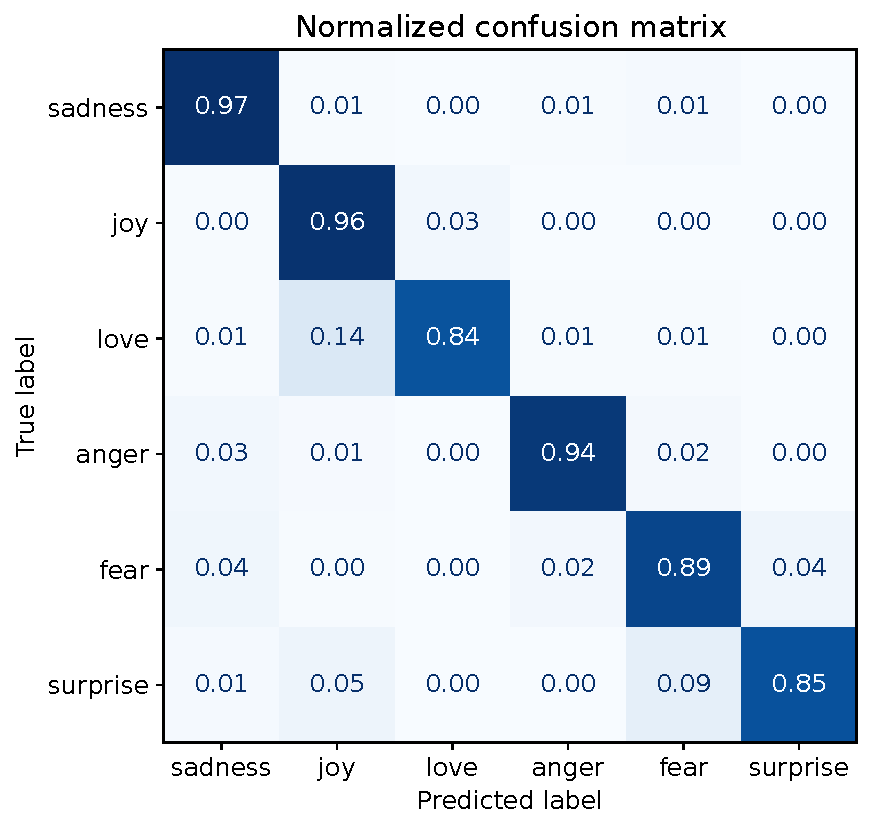
\includegraphics[width=0.8\textwidth]{../figures/finetuned_confusion_matrix.pdf}
  \caption{Normalised confusion matrix of the best fine-tuned model
           on the validation set.  The diagonal entries are close to
           1.0 for most classes, with the primary confusion occurring
           between ``surprise'' and ``joy.''}
  \label{fig:finetuned-confusion}
\end{figure}

\subsection{Adversarial Examples}\label{subsec:adversarial}

We construct five adversarial examples using two complementary strategies.
First, we manually craft two examples designed to exploit specific
weaknesses of Transformer-based classifiers:

\begin{enumerate}
  \item \textbf{Negation scrambling}: A sentence with multiple
    negations (``I'm not unhappy, not upset, and not at all angry'')
    combined with clearly sad context (``terrible news'').  While a
    human reader interprets the intended emotion as sadness, the
    model predicts ``joy,'' demonstrating that multiple negation
    markers confuse the model into ignoring the underlying sentiment.
  \item \textbf{Sarcasm / irony}: A short sarcastic remark
    (``Oh wonderful, just what I needed -- two flat tyres and a
    burnt coffee.'')  The intended emotion is anger, but the model
    predicts ``joy'' with moderate confidence, indicating that it
    relies on surface-level positive words rather than pragmatic
    understanding.
\end{enumerate}

Second, we implement a HotFlip-style gradient-based attack that
automatically searches for token replacements to push a correctly
classified sample toward a target misclassification.  From the
validation set, we collect up to ten high-confidence (score $>0.9$)
correct predictions for each of three classes: ``joy,''
``sadness,'' and ``anger.''  For each class, we take the first
available sample and attempt to push its prediction toward
``love'' using a HotFlip-style gradient attack.  The algorithm
computes the gradient of the target-class loss with respect to the
input embeddings, scores candidate token replacements by their
approximate effect on the loss, and iteratively applies the best
replacement.  Only complete word tokens (not ``\#\#''
subword continuations) are considered.  The attack runs for up to
15 steps with a maximum of 3 replacements; if one candidate fails,
the next from the pool is tried.  Results are summarised in
Table~\ref{tab:adversarial-summary}.

\begin{table}[tbp]
  \centering
  \caption{Summary of five adversarial examples.  ``Source / Target''
           indicates the intended emotion and the misclassification
           goal.  ``Prediction'' is the model's output on the
           adversarial text.}
  \label{tab:adversarial-summary}
  \begin{tabular}{lllc}
    \toprule
    Strategy & Source / Target & Prediction & Success \\
    \midrule
    Negation scrambling & sadness $\rightarrow$ joy & joy & Yes \\
    Sarcasm / irony      & anger  $\rightarrow$ joy & joy & Yes \\
    HotFlip (gradient)   & joy $\rightarrow$ love  & love & Yes \\
    HotFlip (gradient)   & sadness $\rightarrow$ love & love & Yes \\
    HotFlip (gradient)   & anger $\rightarrow$ love & love & Yes  \\
    \bottomrule
  \end{tabular}
\end{table}


%=============================================================================
\section{Conclusion}\label{sec:conclusion}
%=============================================================================

This report presented an emotion recognition system for Twitter text
based on DistilBERT.  Our experiments demonstrate a substantial gap
between feature extraction (~63\%) and fine-tuning (~94\%), confirming
that end-to-end adaptation of pre-trained representations is critical
for downstream text classification tasks.  Error analysis reveals that
class imbalance and vocabulary overlap between ``surprise'' and ``joy''
are the primary causes of misclassification.  Adversarial examples
constructed through both manual crafting and gradient-based attacks
show that the model relies heavily on surface-level token patterns
rather than deeper semantic or pragmatic understanding, leaving it
vulnerable to negation scrambling and sarcasm.

Several limitations should be acknowledged.  The experiments are
limited to a single architecture (DistilBERT) and a single dataset
(CARER emotion).  The grid search, while covering three factors, uses
a relatively coarse grid.  Future work could extend this study by
exploring larger pre-trained models (RoBERTa, DeBERTa), incorporating
adversarial training to improve robustness, and investigating
multi-task learning for joint emotion and sentiment analysis.

\bibliography{references}

\end{document}
